
\section*{Introduction}
\section*{Introduction}
Dans le chapitre précédent, nous avons mis en place la gestion des projets et des contrats, définissant ainsi le cadre contractuel et organisationnel de notre collaboration avec les clients. 
\newline Au cours de ce chapitre, nous présenterons les fonctionnalités constituant le cœur opérationnel de \textbf{SolidMaint} : la gestion des demandes clients et le cycle de vie des tickets de maintenance. Ce troisième sprint se concentre sur l'efficacité du traitement technique, le suivi précis du temps via le chronométrage et le respect rigoureux des engagements de service (SLA).

% ─────────────────────────────────────────────────────────────────────────────
% SECTION 1 : BACKLOG DU SPRINT 1
% ─────────────────────────────────────────────────────────────────────────────
\section{Sprint Planning Meeting }
La planification de ce troisième sprint est cruciale car elle porte sur les fonctionnalités les plus utilisées au quotidien par les clients et les développeurs. L'enjeu est de garantir une transition fluide entre le signalement d'un besoin et sa résolution technique.
L'objectif de ce sprint est de livrer le moteur de production de la plateforme. Cela inclut le module de soumission des demandes pour les clients, l'interface de qualification pour les chefs de projet, et l'environnement de travail des développeurs articulé autour d'un tableau Kanban et d'un système de chronométrage interactif.
\subsubsection{Backlog du premier sprint}
\label{sec:backlog_sprint1}

Voici l’ensemble des fonctionnalités issues du Product Backlog, qui seront réalisées dans le cadre de ce sprint opérationnel.
\newline
\textbf{1 : Effort faible, 2 : Effort moyen, 3 : Effort élevé}
\rowcolors{0}{}{}
\arrayrulecolor{black}
\renewcommand{\arraystretch}{1.3}
\small

\begin{longtable}{|C{1cm}|m{6.5cm}|m{7cm}|C{1cm}|}
\hline
\textbf{ID US} & \textbf{User Story} & \textbf{Description technique} & \textbf{Effort} \\
\hline
\endfirsthead

    \hline

\endhead

\hline
\endfoot

\hline
\endlastfoot

% Epic 1: Authentification et Sécurité
\multicolumn{4}{|l|}{\cellcolor{blue!20}\textbf{Epic 1 - Authentification et Sécurité}} \\
\hline

US01 & En tant qu'\textbf{utilisateur}, je souhaite m'authentifier avec email et mot de passe afin d'accéder à mes informations de manière sécurisée. & 
\vspace{2mm}
\begin{itemize}[nosep, left=0pt, label={$\bullet$}]
\item Développer l'endpoint \texttt{POST /api/auth/login}
\item Mettre en place la gestion de session via \textbf{JWT}
    (access token 15 min, refresh token 7 jours stocké en base)
\item Réaliser l'interface connexion login
\item Consommer l'API d'authentification
\item Gérer les tentatives échouées (3 essais) avec verrouillage temporaire
\end{itemize} & 2 \\
\hline

US02 & En tant qu'\textbf{utilisateur}, je souhaite réinitialiser mon mot de passe afin de retrouver l'accès à mon compte. & 
\vspace{2mm}
\begin{itemize}[nosep, left=0pt, label={$\bullet$}]
\item Développer les endpoints
    \texttt{POST /api/auth/mot-de-passe-oublie} et
    \texttt{POST /api/auth/reinitialiser-mot-de-passe}
  \item Créer les formulaires « mot de passe oublié » et
    de réinitialisation côté Next.js
  \item Générer un token sécurisé (bcrypt) avec expiration
    de \textbf{1 heure}, stocké dans
    \texttt{TokenReinitialisationMotDePasse}
  \item Invalider les anciens tokens non utilisés à chaque
    nouvelle demande
  \item Configurer l'envoi d'un e-mail de réinitialisation
    et d'un e-mail de confirmation via \textbf{Nodemailer}
\end{itemize} & 2 \\
\hline

US03 & En tant qu'\textbf{utilisateur}, je souhaite m'authentifier via Google ou GitHub afin de me connecter rapidement sans créer de compte. & 
\vspace{2mm}
\begin{itemize}[nosep, left=0pt, label={$\bullet$}]
\item Intégrer les stratégies OAuth2 via
    \texttt{passport-google-oauth20} et \texttt{passport-github2}
    dans NestJS (\texttt{@nestjs/passport})
\item Implémenter les routes \texttt{GET /api/auth/google},\texttt{GET /api/auth/github} et leurs callbacks
  \item Si l'utilisateur existe en base et est actif :
    générer les tokens JWT et rediriger vers le frontend
    avec \texttt{?oauth=success}
\item Vérifier l'existence de l'utilisateur en base de données et une demande d'inscription OAuth est envoyée à l'admin
\item Implémenter les routes /auth/google, /auth/github et leurs callbacks, avec génération d'un JWT
\item Implémenter les boutons OAuth sur la page de login
\end{itemize} & 3 \\
\hline

US04 & En tant qu'\textbf{utilisateur}, je souhaite me déconnecter de la plateforme afin de sécuriser ma session. & 
\vspace{2mm}
\begin{itemize}[nosep, left=0pt, label={$\bullet$}]
\item Développer l'endpoint POST /auth/logout avec révocation du refresh token en base
\item Supprimer \texttt{accessToken}, \texttt{refreshToken}
    et \texttt{user} du \texttt{localStorage}
\item Vider le cache React Query (\texttt{queryClient.clear()})
\item Réaliser le bouton de déconnexion 
\end{itemize} & 1 \\
\hline

US05 & En tant qu'\textbf{utilisateur}, je souhaite que mon compte soit protégé contre les tentatives de connexion malveillantes afin de garantir la sécurité de mes données. & 
\vspace{2mm}
\begin{itemize}[nosep, left=0pt, label={$\bullet$}]
  \item Implémenter le compteur de tentatives échouées
    (\texttt{tentativesConnexionEchouees}) en base de données
  \item Verrouiller le compte après \textbf{3 tentatives échouées}
    pendant \textbf{1 minute} via le champ
    \texttt{compteVerrouilleJusquA}
  \item Réinitialiser le compteur à 0 après une connexion réussie
  \item Appliquer le rate limiting global via
    \texttt{@nestjs/throttler} sur les endpoints publics
\end{itemize} & 2 \\
\hline

% Epic 2: Gestion des utilisateurs
\multicolumn{4}{|l|}{\cellcolor{blue!20}\textbf{Epic 2 - Gestion des utilisateurs}} \\
\hline

US06 & En tant qu'\textbf{utilisateur}, je souhaite gérer mon profil afin que mes informations soient toujours à jour. & 
\vspace{2mm}
\begin{itemize}[nosep, left=0pt, label={$\bullet$}]
\item Développer les endpoints \texttt{GET /api/profil} et \texttt{PUT /api/profil}
\item Implémenter l'upload de la photo de profil \texttt{POST /api/profil/upload-photo}
\item Développer le changement de mot de passe via
    \texttt{POST /api/profil/change-password}
    avec vérification de l'ancien mot de passe (bcrypt)
\item Gérer les e-mails secondaires :
    \texttt{GET/POST/DELETE /api/profil/emails} et
    \texttt{PATCH /api/profil/emails/principal}
\item Réaliser l'interface profil côté Next.js  avec formulaire prérempli
\end{itemize} & 2 \\
\hline

US07 & En tant qu'\textbf{administrateur}, je souhaite créer des utilisateurs afin de gérer les accès au système. & 
\vspace{2mm}
\begin{itemize}[nosep, left=0pt, label={$\bullet$}]
\item Développer l'endpoint \texttt{POST /api/users}
\item Générer automatiquement un mot de passe temporaire haché via \textbf{bcrypt} (facteur 10)
\item Générer un token de réinitialisation (1 heure) et construire le lien de réinitialisation
\item Créer automatiquement le \texttt{ProfilEmploye}
    avec matricule \texttt{EMP-\{id\}} si le rôle n'est pas CLIENT
\item Valider les données d'entrée via \textbf{class-validator}
  \item Envoyer un e-mail de bienvenue via \textbf{Nodemailer}
    contenant le mot de passe temporaire et le lien de
    réinitialisation
  \item Réaliser le formulaire d'ajout côté Next.js
\end{itemize} & 3 \\
\hline

US08 & En tant qu'\textbf{administrateur}, je souhaite modifier les informations d'un utilisateur afin de maintenir des données à jour. & 
\vspace{2mm}
\begin{itemize}[nosep, left=0pt, label={$\bullet$}]
\item Développer l'endpoint \texttt{PUT /api/users/:id}
\item Sécuriser l'accès à l'endpoint pour les administrateurs uniquement
\item Valider les données via \textbf{class-validator}
\item Réaliser le formulaire de modification côté Next.js
\end{itemize} & 2 \\
\hline

US09 & En tant qu'\textbf{administrateur}, je souhaite activer et désactiver un compte utilisateur afin de contrôler l'accès au système. & 
\vspace{2mm}
\begin{itemize}[nosep, left=0pt, label={$\bullet$}]
\item Développer les endpoints \texttt{PATCH /api/users/:id/desactiver} et \texttt{PATCH /api/users/:id/reactiver}
\item Implémenter les vérifications de réassignation des tickets et des demandes en cas de désactivation
\item Envoyer des notifications pour informer l'utilisateur de l'activation ou désactivation de son compte
\item Réaliser les boutons d'action avec appels des API
\end{itemize} & 3 \\
\hline

US10 & En tant qu'\textbf{administrateur}, je souhaite consulter la liste des utilisateurs afin de visualiser et gérer efficacement les comptes. & 
\vspace{2mm}
\begin{itemize}[nosep, left=0pt, label={$\bullet$}]
\item Développer l'endpoint \texttt{GET /api/users}
\item Réaliser l'interface d'administration avec vue grille
    et vue liste, filtres par statut et par rôle,
    barre de recherche dynamique

\end{itemize} & 1 \\
\hline

US11 & En tant qu'\textbf{utilisateur}, je souhaite consulter l'historique de mes activités afin de suivre mes actions dans le système. & 
\vspace{2mm}
\begin{itemize}[nosep, left=0pt, label={$\bullet$}]
\item Développer l'endpoint \texttt{GET /api/users/:id/activities} pour récupérer l'historique
\item Implémenter la logique de filtrage dans le backend en utilisant l'opérateur contains
\item Implémenter une barre de recherche dynamique
\item Réaliser l'interface timeline avec filtres par date et type d'action
\end{itemize} & 2 \\
\hline

% Epic 3: Gestion des rôles et permissions
\multicolumn{4}{|l|}{\cellcolor{blue!20}\textbf{Epic 3 - Gestion des rôles et permissions}} \\
\hline

US12 & En tant qu'\textbf{administrateur}, je souhaite gérer des rôles afin de structurer les accès au système. & 
\vspace{2mm}
\begin{itemize}[nosep, left=0pt, label={$\bullet$}]
\item Développer les endpoints CRUD pour la gestion complète des rôles
\item Implémenter le PermissionsGuard et le décorateur @Permissions pour sécuriser les routes du backend 
\item Réaliser l'interface de gestion sous forme de matrice
\end{itemize} & 3 \\
\hline

US13 & En tant qu'\textbf{administrateur}, je souhaite attribuer des permissions granulaires aux rôles afin de contrôler précisément les accès. & 
\vspace{2mm}
\begin{itemize}[nosep, left=0pt, label={$\bullet$}]
\item Développer l’endpoint PATCH /roles-permissions/roles/:id/sync pour synchroniser dynamiquement les associations entre un rôle et ses permissions. 
\item Implémenter la logique de mise à jour atomique                                                                                                                                                                                                                       
\item Développer l'interface interactive de type "Matrice de contrôle d'accès" 

\end{itemize} & 2 \\
\hline
US14 & En tant qu'\textbf{administrateur}, je souhaite consulter la matrice rôles-permissions afin de visualiser rapidement les droits de chaque rôle. & 
\vspace{2mm}
\begin{itemize}[nosep, left=0pt, label={$\bullet$}]
\item Développer l’endpoint GET /roles-permissions/matrix ) pour récupérer les données 
\item Implémenter la logique de structuration des données au format JSON                
\item Réaliser l’interface de visualisation de type "Heatmap" ou "Tableau de bord"

\end{itemize} & 3 \\
\hline

% Epic 4: Demandes d'inscription OAuth
\multicolumn{4}{|l|}{\cellcolor{blue!20}\textbf{Epic 4 - Demandes d'inscription OAuth}} \\
\hline

US15 & En tant qu'\textbf{utilisateur externe}, je souhaite demander l'accès via OAuth afin de m'inscrire facilement. & 
\vspace{2mm}
\begin{itemize}[nosep, left=0pt, label={$\bullet$}]
\item Développer l'endpoint POST /auth/oauth/request pour créer une demande
\item Enregistrer la demande en base avec statut EN\_ATTENTE
\item Implémenter l'envoi de notification à l'administrateur via email et in-app
\item Réaliser l'interface de demande d'accès
\end{itemize} & 3 \\
\hline

US16 & En tant qu'\textbf{administrateur}, je souhaite valider ou rejeter les demandes d'inscription OAuth afin de contrôler les accès. & 
\vspace{2mm}
\begin{itemize}[nosep, left=0pt, label={$\bullet$}]
\item Développer les endpoints PATCH /auth/oauth/requests/:id/approve et /reject
\item Implémenter la création automatique du compte utilisateur lors de l'approbation
\item Configurer l'envoi d'emails de confirmation ou rejet via Nodemailer
\item Réaliser l'interface de gestion des demandes avec actions d'approbation/rejet
\end{itemize} & 3 \\
\hline
% Epic 4: Demandes d'inscription OAuth


\end{longtable}



% ─────────────────────────────────────────────────────────────────────────────
% SECTION 2 : ANALYSE
% ─────────────────────────────────────────────────────────────────────────────

\section{Analyse}
Dans cette phase, nous traduisons les besoins opérationnels en spécifications techniques, en mettant l'accent sur les transitions de statuts et les règles de gestion du temps de travail.
\subsection{Diagramme des cas d'utilisation du troisième sprint}
La figure ci-dessous présente le diagramme de cas d’utilisation du troisième sprint, centré sur le flux de traitement des incidents :
\begin{figure}[H]
        \centering
        \includegraphics[width=0.85\textwidth,height=0.60\textheight,keepaspectratio]{Images/Diagramme_cas_utilisation_sprint3.png}
        \caption{Diagramme des cas d'utilisation du troisième sprint}
        \label{fig:use_case_sprint3}
\end{figure}
\subsection{Description textuelle du cas d'utilisation « Convertir demande en ticket »}
Ce cas d'utilisation est le point de pivot entre le client et l'équipe technique.
\begin{table}[H]
\centering
\footnotesize
\renewcommand{\arraystretch}{1}
\begin{tabular}{|p{4.5cm}|p{12cm}|}
\hline
\textbf{Nom du cas d'utilisation} & Convertir une demande en ticket \\
\hline
\textbf{Acteurs} & Chef de projet \\
\hline
\textbf{Préconditions} & Une demande client est au statut \textit{EN\_ATTENTE} \\
\hline
\textbf{Postconditions} & Un ticket est créé, lié à la demande initiale, et les SLA sont initialisés \\
\hline
\textbf{Scénario principal} &
\begin{minipage}[t]{\linewidth}
\begin{enumerate}[label=\arabic*., nosep,leftmargin=0.8cm,topsep=0pt,itemsep=2pt]
\item Le Chef de projet accède à la liste des demandes en attente.
\item Il sélectionne une demande pour examiner son contenu et les pièces jointes.
\item Il valide la demande en définissant la priorité (Mineur, Majeur, Critique) et le type de maintenance.
\item Le système crée automatiquement le ticket avec un numéro de suivi unique.
\item Le système calcule les dates d'échéance selon la configuration SLA du contrat associé.
\item Le système notifie le client du passage en traitement technique.
\end{enumerate}
\vspace{2pt}
\end{minipage} \\
\hline
\textbf{Scénarios d'exception} &
\begin{itemize}[nosep,leftmargin=0.8cm,topsep=0pt,itemsep=2pt, label=$\bullet$]
\item La demande est incomplète : le CP demande des informations complémentaires (statut \textit{INFOS\_REQUISES}).
\item La demande est hors périmètre : le CP rejette la demande avec un motif obligatoire.
\end{itemize} \\
\hline
\end{tabular}
\caption{Description textuelle du cas « Convertir demande en ticket »}
\end{table}
\subsection{Description textuelle du cas d'utilisation « Gérer le chronomètre »}
Ce cas d'utilisation permet un suivi granulaire de l'effort fourni sur chaque ticket.
\begin{table}[H]
\centering
\footnotesize
\renewcommand{\arraystretch}{1}
\begin{tabular}{|p{4.5cm}|p{12cm}|}
\hline
\textbf{Nom du cas d'utilisation} & Gérer le chronomètre de travail \\
\hline
\textbf{Acteurs} & Développeur \\
\hline
\textbf{Préconditions} & Le développeur est assigné au ticket et celui-ci est au statut \textit{OUVERT} ou \textit{EN\_COURS} \\
\hline
\textbf{Postconditions} & Une session de travail est enregistrée et le temps passé sur le ticket est cumulé \\
\hline
\textbf{Scénario principal} &
\begin{minipage}[t]{\linewidth}
\begin{enumerate}[label=\arabic*., nosep,leftmargin=0.8cm,topsep=0pt,itemsep=2pt]
\item Le développeur ouvre la vue détail du ticket assigné.
\item Il clique sur le bouton « Démarrer » pour lancer le suivi.
\item Le système enregistre l'heure précise de début et change le statut du ticket à \textit{EN\_COURS}.
\item Le développeur effectue ses tâches techniques.
\item Il clique sur « Arrêter » une fois l'intervention terminée ou pour faire une pause.
\item Le système calcule la durée de la session, l'ajoute au total du ticket et clôture la session de travail.
\end{enumerate}
\vspace{2pt}
\end{minipage} \\
\hline
\textbf{Scénarios d'exception} &
\begin{itemize}[nosep,leftmargin=0.8cm,topsep=0pt,itemsep=2pt, label=$\bullet$]
\item Le développeur oublie de couper le chrono : il peut modifier manuellement la durée avec une justification (traçabilité).
\end{itemize} \\
\hline
\end{tabular}
\caption{Description textuelle du cas « Gérer le chronomètre »}
\end{table}
% ─────────────────────────────────────────────────────────────────────────────
% SECTION 3 : CONCEPTION
% ─────────────────────────────────────────────────────────────────────────────
\section{Conception}
La conception du Sprint 3 s'appuie sur une modélisation rigoureuse des transitions de statuts et de la logique temporelle.
\subsection{Diagramme de classes du troisième sprint}
Le diagramme suivant détaille la structure des entités \texttt{Ticket}, \texttt{Demande}, et \texttt{SessionTravail}, ainsi que leurs relations avec les contrats (SLA).
\begin{figure}[H]
        \centering
        \includegraphics[width=1\textwidth,keepaspectratio]{Images/diag_classe_sprint3.png}
        \caption{Diagramme de classes du Sprint 3 - Cœur opérationnel}
        \label{fig:diag_classe_sprint3}
\end{figure}
\section{Diagramme de séquence}
\subsection{Diagramme de séquences du cas d'utilisation « Conversion Demande en Ticket »}
Ce diagramme illustre le processus de validation métier et la création automatisée des entités techniques.
\begin{figure}[H]
        \centering
        \includegraphics[width=0.75\textwidth,keepaspectratio]{Images/diag_seq_conversion.png}
        \caption{Diagramme de séquence du cas « Conversion Demande en Ticket »}
        \label{fig:seq_conversion}
\end{figure}
\subsection{Diagramme de séquences du cas d'utilisation « Signalement de blocage »}
Ce diagramme détaille comment un signalement de blocage par un développeur suspend automatiquement le décompte du délai SLA.
\begin{figure}[H]
        \centering
        \includegraphics[width=0.75\textwidth,keepaspectratio]{Images/diag_seq_blocage.png}
        \caption{Diagramme de séquence du cas « Signalement de blocage »}
        \label{fig:seq_blocage}
\end{figure}
\section{Schéma relationnel}
\textbf{Ticket} (\underline{idTicket}, \textbf{\#idDemande}, titre, description, statut, priorite, type, \textbf{\#idProjet}, dateEcheanceSLA, tempsEstime)
\newline
\textbf{SessionTravail} (\underline{idSession}, \textbf{\#idTicket}, \textbf{\#idUtilisateur}, dateDebut, dateFin, dureeSecondes, descriptionTravail)
\newline
\textbf{DemandeClient} (\underline{idDemande}, \textbf{\#idProfilC}, titre, description, statut, dateCreation, \textbf{\#idContrat})
\newline
\textbf{TicketBlocage} (\underline{idBlocage}, \textbf{\#idTicket}, raison, statutBlocage, dateSignalement, dateResolution)
% ─────────────────────────────────────────────────────────────────────────────
% SECTION 4 : RÉALISATION
% ─────────────────────────────────────────────────────────────────────────────
\section{Réalisation}
Après avoir analysé les besoins et conçu les solutions, nous passons maintenant à la réalisation. Dans cette phase, nous avons développé toutes les user stories planifiées dans le sprint backlog. Cette section présente le diagramme de composants qui montre l'architecture de notre application, ainsi que les interfaces utilisateur que nous avons créées pour répondre aux besoins des utilisateurs.
\label{sec:realisation_sprint1}

\subsection{Diagramme de composants}


\subsection{Description des interfaces}
Cette section présente les principales interfaces utilisateur développées lors du premier sprint.

\subsubsection{Interface de connexion}
\begin{figure}[H]
\centering
%\includegraphics[width=0.75\textwidth,keepaspectratio]{Images/interface_connexion.png}
\caption{Interface de connexion — authentification classique et OAuth}
\label{fig:interface_connexion}
\end{figure}
La page de connexion propose deux modes d'authentification : le formulaire
classique (e-mail + mot de passe) et les boutons OAuth (Google, GitHub).
En cas de compte inexistant, le visiteur est redirigé vers un flux de
demande d'inscription.

\subsubsection{Interface de réinitialisation du mot de passe}
\begin{figure}[H]
\centering
%\includegraphics[width=0.75\textwidth,keepaspectratio]{Images/interface_reset_password.png}
\caption{Interface de réinitialisation du mot de passe}
\label{fig:interface_reset}
\end{figure}
Cette interface permet à l'utilisateur de saisir son adresse e-mail pour
recevoir un lien de réinitialisation valable 1 heure.

\subsubsection{Interface de gestion des utilisateurs}
\begin{figure}[H]
\centering
%\includegraphics[width=0.85\textwidth,keepaspectratio]{Images/interface_users.png}
\caption{Interface d'administration — liste des utilisateurs}
\label{fig:interface_users}
\end{figure}
L'administrateur dispose d'une vue en grille ou en liste, avec filtres par
statut et par rôle, barre de recherche et actions rapides (modifier,
désactiver, voir le profil).

\subsubsection{Interface de gestion des rôles et permissions}
\begin{figure}[H]
\centering
%\includegraphics[width=0.85\textwidth,keepaspectratio]{Images/interface_roles_permissions.png}
\caption{Interface d'administration — gestion des rôles et permissions}
\label{fig:interface_roles}
\end{figure}
La matrice des permissions affiche les rôles en colonnes et les catégories
de permissions en lignes, avec des cases à cocher pour une attribution
visuelle et intuitive.

\subsubsection{Interface de gestion des demandes d'inscription OAuth}
\begin{figure}[H]
\centering
%\includegraphics[width=0.85\textwidth,keepaspectratio]{Images/interface_demandes_oauth.png}
\caption{Interface d'administration — demandes d'inscription OAuth}
\label{fig:interface_oauth}
\end{figure}
L'administrateur consulte les demandes en attente, visualise les
informations récupérées via OAuth et peut approuver ou refuser chaque
demande avec un motif de refus facultatif.

% ─────────────────────────────────────────────────────────────────────────────
% SECTION 5 : TESTS
% ─────────────────────────────────────────────────────────────────────────────
\section{Tests et Validation}
La phase de test est essentielle pour garantir la qualité et la fiabilité de la solution. Elle valide que chaque fonctionnalité répond aux exigences métier et identifie les anomalies avant la mise en production. Dans ce sprint, nous avons testé les mécanismes d'authentification, la gestion des utilisateurs et le contrôle d'accès (RBAC) pour assurer la robustesse de nos implémentations.

\subsection{Stratégie de tests adoptée}
Afin de garantir la qualité et la fiabilité de l'application, nous avons adopté une stratégie de tests structurée, reposant sur une répartition des vérifications à plusieurs niveaux. Cette approche permet d'assurer une bonne couverture fonctionnelle avec un temps d'exécution raisonnable, tout en facilitant l'identification rapide des anomalies.

Les tests ont été organisés par module fonctionnel afin d'assurer une meilleure traçabilité des vérifications effectuées. Ainsi, les tests unitaires couvrent les règles métier les plus fines, les tests d'intégration valident les échanges avec l'API, et les tests End-to-End reproduisent les scénarios complets d'utilisation de l'application.

La pyramide de tests se compose donc de trois niveaux complémentaires :


\subsubsection{Tests unitaires}
\label{sec:tests_unitaires}

Les tests unitaires ont été réalisés à l'aide du framework \textbf{Vitest},
en isolant chaque service du reste de l'application grâce à des mocks
Prisma. Cette approche garantit l'indépendance des tests et permet une
détection précoce des anomalies dès la phase de développement. Trois
modules prioritaires ont été couverts : l'authentification, le contrôle
d'accès basé sur les rôles (RBAC) et la gestion des clients.

\vspace{4pt}
\noindent\textbf{Bilan : 45 tests exécutés — 45 réussis — 0 échec.}
\vspace{6pt}

\begin{itemize}[leftmargin=0pt]

% ── 1. Authentification ───────────────────────────────────────────────────────
\item[$\square$] \textbf{Module Authentification}
\hfill\textit{Méthodes : \texttt{login()} ·
\texttt{demanderReinitialisationMotDePasse()} ·
\texttt{reinitialiserMotDePasse()}}

\noindent Cette suite valide le processus d'authentification classique,
la génération des jetons JWT et le mécanisme de réinitialisation du mot
de passe. Les cas suivants ont été couverts :

\begin{itemize}[label=$\bullet$, nosep, itemsep=2pt]
  \item Un utilisateur actif fournit des identifiants valides : les jetons
    \texttt{accessToken} et \texttt{refreshToken} sont générés
    correctement.
  \item L'adresse e-mail fournie n'existe pas en base de données : la
    connexion est rejetée avec le code \texttt{401 Unauthorized}.
  \item Le mot de passe fourni est incorrect : la connexion est rejetée
    avec le code \texttt{401 Unauthorized}.
  \item L'utilisateur échoue l'authentification \textbf{3 fois
    consécutives} : le compte est verrouillé automatiquement pendant
    \textbf{1 minute} (\texttt{maxLoginAttempts = 3}).
  \item L'utilisateur tente de se connecter alors que son compte est
    verrouillé : la connexion est rejetée avec un message explicite.
  \item Le compte de l'utilisateur est désactivé : la connexion est
    rejetée avec le code \texttt{401 Unauthorized}.
  \item L'adresse e-mail fournie pour la réinitialisation est inexistante :
    une \texttt{NotFoundException} est levée.
  \item Le token de réinitialisation a été généré depuis plus d'une heure :
    une \texttt{BadRequestException} est levée.
\end{itemize}

% ── 2. RBAC ───────────────────────────────────────────────────────────────────
\item[$\square$] \textbf{Module Gestion des rôles et permissions (RBAC)}
\hfill\textit{Méthodes : \texttt{creerPermission()} ·
\texttt{attribuerRoleUtilisateur()} ·
\texttt{obtenirRolesEtPermissions()}}

\noindent Cette suite valide les règles d'exclusivité des rôles, l'unicité
des permissions et l'intégrité des références. Les cas suivants ont été
couverts :

\begin{itemize}[label=$\bullet$, nosep, itemsep=2pt]
  \item Une permission est créée avec un code unique : elle est enregistrée
    correctement en base de données.
  \item Une permission est créée avec un code déjà existant : une
    \texttt{BadRequestException} est levée.
  \item Les rôles et permissions d'un utilisateur sont récupérés : la liste
    est retournée sans doublons.
  \item Un rôle est attribué à un utilisateur sans rôle existant :
    l'attribution est réussie.
  \item L'utilisateur cible est inexistant : une \texttt{NotFoundException}
    est levée.
  \item La règle d'exclusivité \texttt{CLIENT} et \texttt{CHEF\_PROJET}
    est violée : une \texttt{BadRequestException} est levée.
  \item La règle d'exclusivité \texttt{CLIENT} et \texttt{DEVELOPPEUR}
    est violée : une \texttt{BadRequestException} est levée.
  \item La règle d'exclusivité \texttt{CLIENT} et \texttt{ADMIN} est
    violée : une \texttt{BadRequestException} est levée.
  \item La combinaison \texttt{ADMIN} et \texttt{CHEF\_PROJET} est
    soumise : l'attribution est \textbf{autorisée} et réussie.
  \item Le rôle est déjà attribué à l'utilisateur : une
    \texttt{BadRequestException} est levée (doublon détecté).
  \item Le rôle à attribuer est inexistant : une \texttt{NotFoundException}
    est levée.
\end{itemize}

% ── 3. Gestion des clients ────────────────────────────────────────────────────
\item[$\square$] \textbf{Module Gestion des clients}
\hfill\textit{Méthodes : \texttt{mettreAJourClient()} ·
\texttt{desactiverClient()} · \texttt{reactiverClient()} ·
\texttt{telechargerLogo()} · \texttt{supprimerLogo()}}

\noindent Cette suite valide les opérations de gestion des clients,
la gestion des fichiers logo et le service de géocodage. Les cas suivants
ont été couverts :

\begin{itemize}[label=$\bullet$, nosep, itemsep=2pt]
  \item Les informations d'un client existant sont mises à jour : le
    résultat validé est retourné correctement.
  \item La mise à jour est effectuée sur un client inexistant : une
    \texttt{NotFoundException} est levée.
  \item Un client actif est désactivé : l'opération est réalisée avec
    succès.
  \item Un client désactivé est réactivé : l'opération est réalisée avec
    succès.
  \item La réactivation est effectuée sur un client inexistant : une
    \texttt{NotFoundException} est levée.
  \item Un logo est téléversé pour un client existant : le fichier est
    traité et stocké correctement.
  \item Le logo d'un client est supprimé : un message de succès est
    retourné.
  \item Le téléversement ou la suppression du logo est effectué sur un
    client inexistant : une \texttt{NotFoundException} est levée.
  \item Le service de géocodage est interrogé avec une adresse valide
    présente en cache : l'adresse est retournée correctement.
  \item Le service de géocodage est interrogé avec une requête trop courte :
    un tableau vide est retourné.
  \item Les résultats du service de géocodage sont mis en cache
    correctement après la première requête.
  \item Les résultats filtrés du géocodage éliminent les doublons de type
    pays.
\end{itemize}

\end{itemize}

\begin{figure}[H]
\centering
\begin{minipage}{0.48\textwidth}
  \centering
  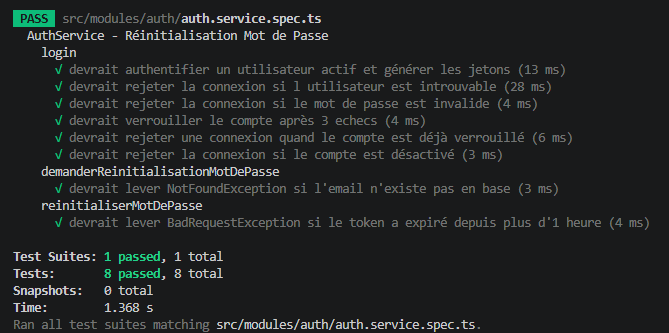
\includegraphics[width=\textwidth,keepaspectratio]
    {Images/test-unitaire-auth.png}
  \caption*{\small Auth}
\end{minipage}
\hfill
\begin{minipage}{0.48\textwidth}
  \centering
  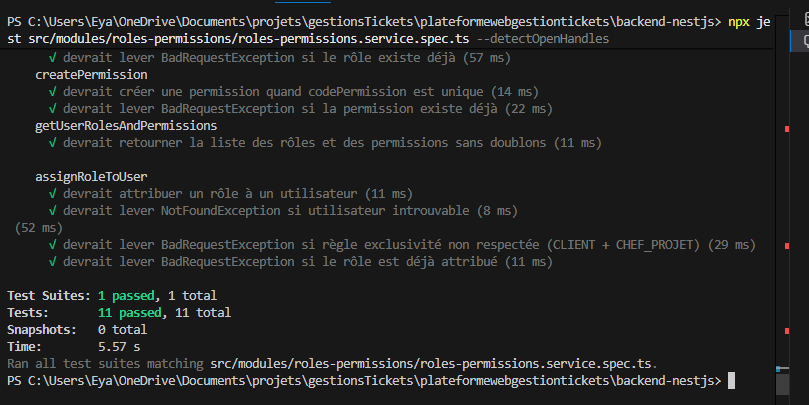
\includegraphics[width=\textwidth,keepaspectratio]
    {Images/test-sprint1-moduleRole+Permession.png}
  \caption*{\small RBAC}
\end{minipage}
\caption{Résultats des tests unitaires — Auth et RBAC}
\label{fig:test_unitaires}
\end{figure}

\begin{figure}[H]
\centering
\begin{minipage}{0.6\textwidth}
  \centering
  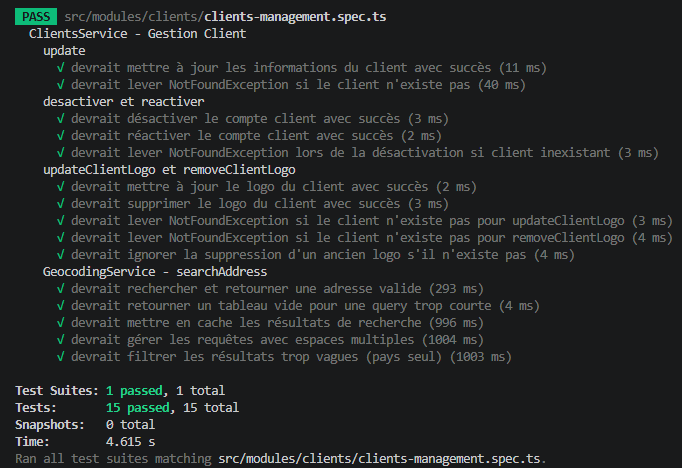
\includegraphics[width=\textwidth,keepaspectratio]
    {Images/test unit-ClientTestUnitaire.png}
  \caption*{\small Gestion des clients}
\end{minipage}
\caption{Résultats des tests unitaires — Gestion des clients}
\end{figure}

% \subsubsection{Tests de sécurité}
% \label{sec:tests_securite}

% Ces tests valident que les mécanismes de protection résistent aux accès
% non autorisés et aux tentatives d'attaque. Ils sont effectués via
% \textbf{Swagger} en combinaison avec les tests unitaires existants.

% \vspace{4pt}
% \noindent\textbf{4 tests exécutés — 4 réussis — 0 échec.}
% \vspace{6pt}

% \begin{itemize}[leftmargin=0pt]

% \item[$\square$] \textbf{Contrôle d'accès aux endpoints protégés}
% \hfill\textit{Guard \texttt{JwtAuthGuard} · \texttt{PermissionsGuard}}

% \begin{itemize}[label=$\bullet$, nosep, itemsep=1pt]
%   \item \texttt{GET /api/auth/me} sans token Bearer →
%     \textbf{401 Unauthorized}.
%   \item \texttt{GET /api/admin/users} avec token CLIENT →
%     \textbf{403 Forbidden}
%     (permission \texttt{users.read.all} absente).
%   \item \texttt{POST /api/admin/roles} avec token DEVELOPPEUR →
%     \textbf{403 Forbidden}
%     (permission \texttt{roles.create} absente).
%   \item Token JWT expiré (après 15 min) →
%     \textbf{401 Unauthorized}, rafraîchissement automatique déclenché
%     côté frontend (intercepteur Axios).
% \end{itemize}

% \vspace{6pt}
% \item[$\square$] \textbf{Protection contre le bruteforce}
% \hfill\textit{\texttt{maxLoginAttempts = 3} ·
% \texttt{lockDurationMs = 60\,000 ms}}

% \begin{itemize}[label=$\bullet$, nosep, itemsep=1pt]
%   \item \textbf{3 tentatives échouées} consécutives → champ
%     \texttt{compteVerrouilleJusquA} mis à jour en base, connexion
%     bloquée \textbf{1 minute}.
%   \item Tentative sur compte verrouillé avant expiration → rejetée
%     immédiatement, sans vérification du mot de passe.
% \end{itemize}

% \end{itemize}

% \begin{figure}[H]
% \centering
% \includegraphics[width=0.72\textwidth,keepaspectratio]
%   {Images/test-securite-acces.png}
% \caption{Tests de sécurité — Contrôle d'accès et protection bruteforce
%   via Swagger}
% \label{fig:test_securite}
% \end{figure}

\subsubsection{Tests d'intégration}
\label{sec:tests_integration}

Les tests d'intégration ont pour objectif de valider les échanges entre
les différentes couches de l'application (contrôleur, service et base de
données) en testant les endpoints REST dans leur ensemble. Ces tests sont
effectués via \textbf{Swagger UI} en soumettant des requêtes HTTP réelles
contre le backend en cours d'exécution, ce qui permet de vérifier le
comportement de l'API dans des conditions proches de la production.

\vspace{4pt}
\noindent\textbf{Bilan : 5 tests exécutés — 5 réussis — 0 échec.}
\vspace{6pt}

\begin{itemize}[leftmargin=0pt]

\item[$\square$] \textbf{Authentification}
\hfill\textit{Endpoint : \texttt{POST /api/auth/login}}

\noindent Cette suite valide le comportement complet de l'endpoint de
connexion, notamment le retour des jetons d'authentification, des rôles,
des permissions associées et la gestion des codes d'erreur HTTP selon les
différents cas d'entrée. Les cas suivants ont été couverts :

\begin{itemize}[label=$\bullet$, nosep, itemsep=2pt]
  \item Un utilisateur actif de rôle \texttt{ADMIN} fournit des
    identifiants valides : l'endpoint retourne le code \textbf{200 OK}
    accompagné des champs \texttt{accessToken}, \texttt{refreshToken},
    des données de l'utilisateur, de ses rôles et de la liste complète
    de ses permissions.
  \item L'adresse e-mail fournie n'existe pas en base de données :
    l'endpoint retourne le code \textbf{401 Unauthorized}.
  \item Le mot de passe fourni est incorrect : l'endpoint retourne le
    code \textbf{401 Unauthorized}.
  \item Les données soumises sont invalides (adresse e-mail mal formatée
    ou champ obligatoire vide) : l'endpoint retourne le code
    \textbf{400 Bad Request} accompagné d'un message de validation
    généré par \texttt{class-validator}.
  \item Le compte de l'utilisateur est désactivé
    (\texttt{estActif = false}) : l'endpoint retourne le code
    \textbf{401 Unauthorized} avec le message
    « Ce compte est désactivé ».
\end{itemize}

\end{itemize}

\begin{figure}[H]
\centering
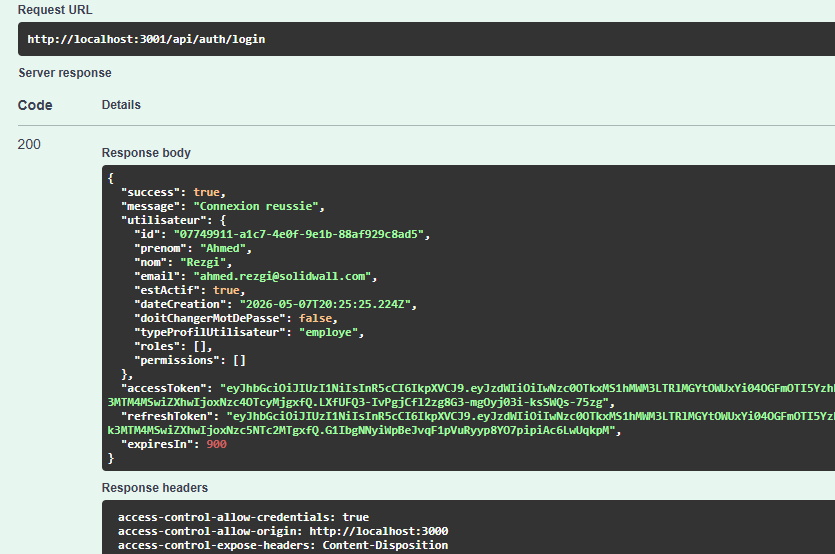
\includegraphics[width=0.60\textwidth,keepaspectratio]
  {Images/test-interg-login.png}
\caption{Test d'intégration — endpoint \texttt{POST /api/auth/login}
  via Swagger}
\label{fig:test_integration}
\end{figure}

%─────────────────────────────────────────────────────────────────────────────
\newpage
%─────────────────────────────────────────────────────────────────────────────
\subsubsection{Tests End-to-End}
\label{sec:tests_e2e}

Les tests End-to-End ont pour objectif de simuler les parcours utilisateurs
complets dans un navigateur réel piloté par \textbf{Playwright}. Ces tests
s'exécutent en interaction avec le frontend Next.js, le backend NestJS et
la base de données PostgreSQL, reproduisant ainsi les conditions réelles
d'utilisation de la plateforme.

\vspace{4pt}
\noindent\textbf{Bilan : 11 tests exécutés — 11 réussis — 0 échec.}
\vspace{6pt}

\begin{itemize}[leftmargin=0pt]

% ── 1. Authentification ───────────────────────────────────────────────────────
\item[$\square$] \textbf{Authentification}
\hfill\textit{10 scénarios : connexion classique, OAuth, déconnexion}

\noindent Cette suite valide le flux complet d'authentification en
simulant les actions réelles d'un utilisateur sur l'interface. Les cas
suivants ont été couverts :

\begin{itemize}[label=$\bullet$, nosep, itemsep=2pt]
  \item La page de connexion est chargée : le formulaire et les boutons
    d'authentification OAuth sont affichés correctement.
  \item Les champs du formulaire sont vides ou partiellement remplis :
    le bouton de soumission reste désactivé.
  \item L'utilisateur soumet des identifiants valides : le flux aboutit
    à une redirection vers la page d'accueil et une session est créée.
  \item L'utilisateur saisit un identifiant ou un mot de passe invalide :
    un message d'erreur approprié est affiché sans redirection.
  \item L'utilisateur échoue l'authentification \textbf{3 fois
    consécutives} : le compte est verrouillé pendant \textbf{1 minute}
    et un message d'information est affiché.
  \item L'utilisateur se déconnecte : les jetons sont supprimés du
    \texttt{localStorage} et l'utilisateur est redirigé vers la page
    \texttt{/connexion}.
  \item L'utilisateur s'authentifie via \textbf{Google} avec succès :
    les données du profil sont récupérées et une session valide est
    créée.
  \item L'authentification via \textbf{Google} échoue : un message
    d'erreur technique est affiché.
  \item L'utilisateur s'authentifie via \textbf{GitHub} avec succès :
    les données du profil sont récupérées et une session valide est
    créée.
  \item L'authentification via \textbf{GitHub} échoue : un message
    d'erreur technique est affiché.
\end{itemize}

\begin{figure}[H]
\centering
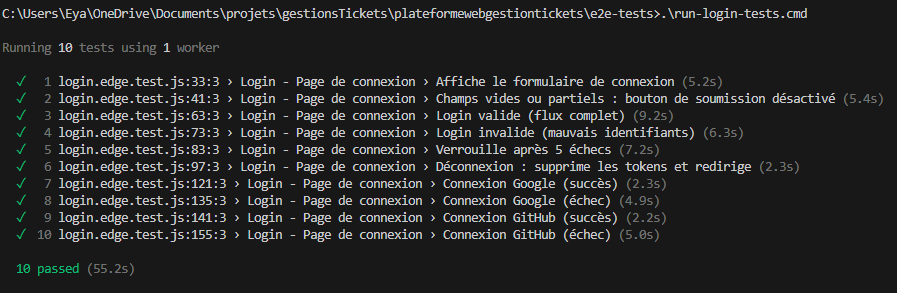
\includegraphics[width=0.68\textwidth,keepaspectratio]
  {Images/ExecDeTestCasesReussi-auth.png}
\caption{Tests End-to-End — Authentification via Playwright}
\label{fig:test_e2e_auth}
\end{figure}

% ── 2. Désactivation utilisateur ─────────────────────────────────────────────
\item[$\square$] \textbf{Gestion des utilisateurs}
\hfill\textit{1 scénario : désactivation avec réassignation des tickets}

\noindent Cette suite valide le flux complet de désactivation d'un
utilisateur disposant de tickets actifs, en simulant les actions réelles
d'un administrateur. Le cas suivant a été couvert :

\begin{itemize}[label=$\bullet$, nosep, itemsep=2pt]
  \item L'administrateur tente de désactiver un utilisateur actif
    disposant de \textbf{9 tickets actifs} (statuts \texttt{OUVERT},
    \texttt{EN\_COURS} ou \texttt{EN\_REVUE}) : le système affiche le
    modal de réassignation présentant la liste des développeurs
    disponibles \textbf{triés par charge de travail croissante}.
    L'administrateur procède à la réassignation de chaque ticket, puis
    confirme l'opération via le bouton « Réassigner et Désactiver ».
    Le système effectue les réassignations dans une transaction atomique,
    désactive le compte et envoie un e-mail de notification à
    l'utilisateur concerné.
\end{itemize}

\begin{figure}[H]
\centering
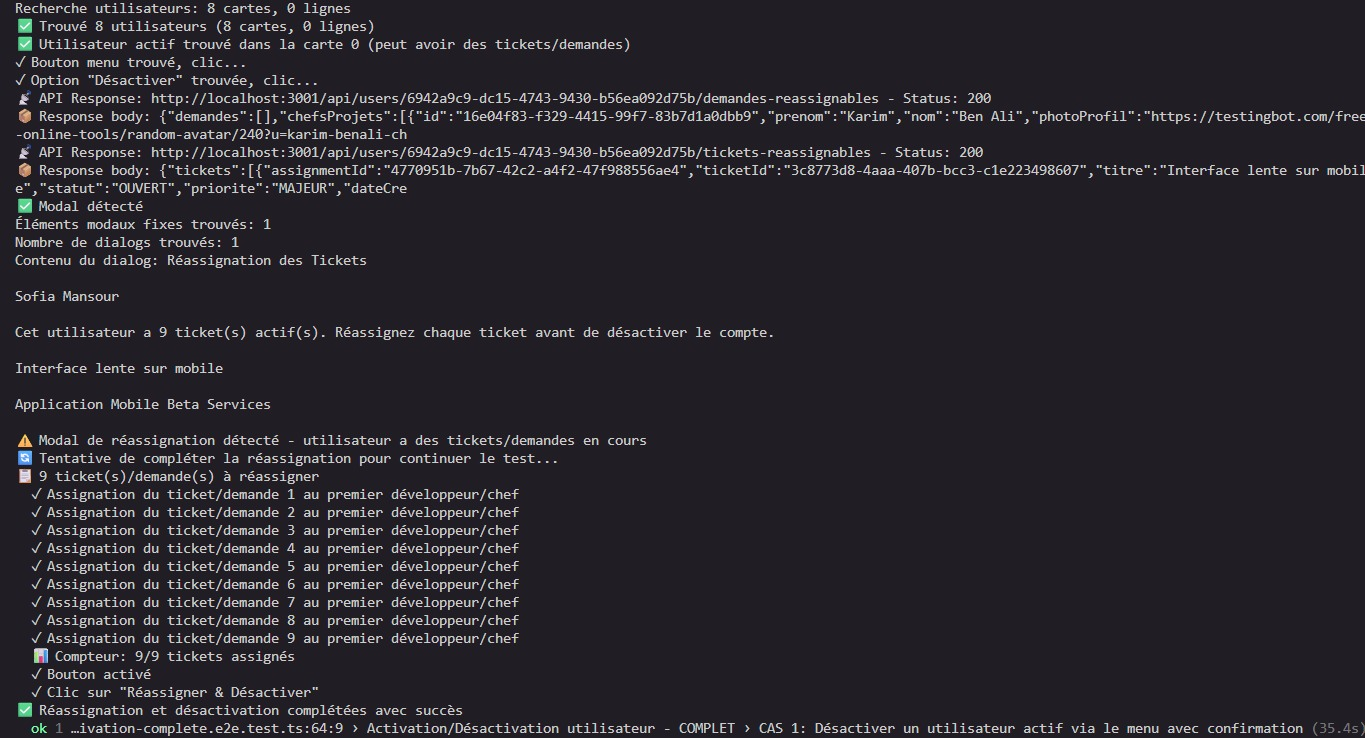
\includegraphics[width=0.68\textwidth,keepaspectratio]
  {Images/Test e2e desactiver utilisateu.png}
\caption{Tests End-to-End — Désactivation utilisateur via Playwright}
\label{fig:test_e2e_desactiver}
\end{figure}

\end{itemize}
